\section{Iteration 2}
Der in der ersten Iteration erstellte Prototyp wurde dem Auftraggeber in Form eine Demo gezeigt.
Dabei sind folgenden Rückmeldungen entstanden:
\begin{itemize}
    \item Der Prototyp entspricht den Vorstellungen und erfüllt die definierten Anforderungen.
    \item Die Vorgabe, dass die Benutzerschnittstelle für Mobilgeräte ausgelegt sein soll, fällt weg.
          Sie soll nur für Desktop-Geräte ausgelegt sein.
    \item Nebst Spannungswerten soll die Applikation auch Leistungs- und \ac{THD} Werte verarbeiten können.
    \item Bisher wurden sämtliche Daten künstlich erstellt.
    Diese sollen um echte Messwerte erweiter werden, welche von Auftraggeber zur Verfügung gestellt werden.
    \item Die Benutzerschnittstelle soll um die Funktion erweitert werden,
    dass eine spezifische Zeitspanne ausgewählt werden kann.



\end{itemize}

\subsection{\ac{MQTT} Datenverarbeitung}

Da neu auch die Leistungs- und \ac{THD} Werte der Stromzähler verarbeitet werden sollen, wurde
die \ac{MQTT} Datenverarbeitung angepasst. Der Dataingress erwartet nun, dass nebst
den Spannungen der drei Phasen auch noch die Leistung und der \ac{THD} Wert mitgeschickt wird.

Dazu wurde auch das Datenbankschema so angepasst, dass die neuen Daten abgespeichert
werden können. Zudem wurden die Tests so angepasst, dass sie auch diese Daten
mitsenden.

\begin{figure}[h]
    \centering
    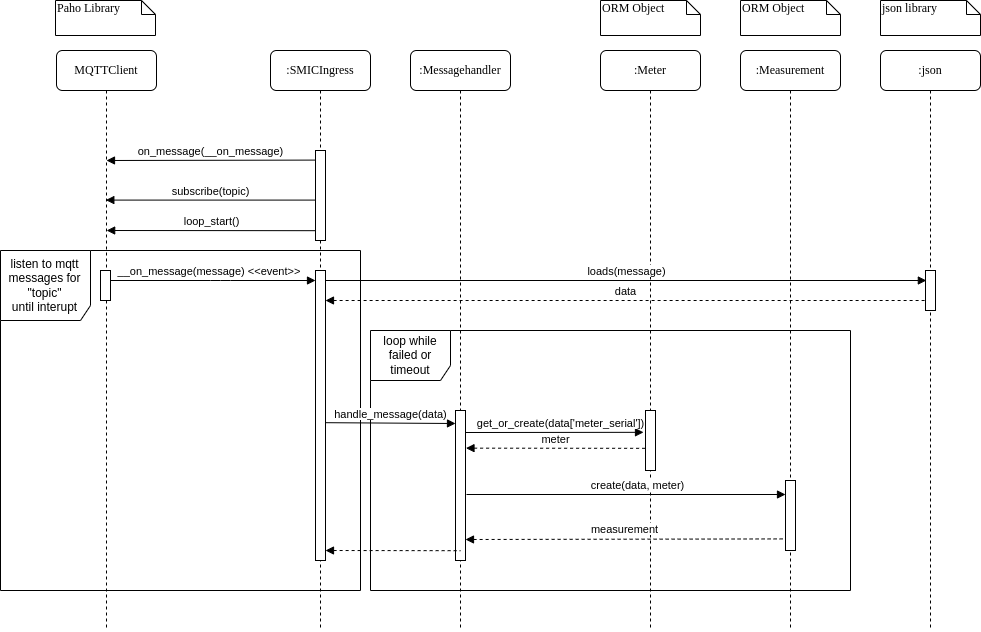
\includegraphics[width=1.0\textwidth]{gfx/dataingress-sequence}
    \caption{
        Impelemtation von Errorhandling durch den Messagehandler und einen
        retry loop.
    }
    \label{fig:dataingress-sequence}
\end{figure}

Bei der Entwicklung zeigte sich zudem, dass der Dataingress nicht sehr stabil
funktioniert und sporadisch fehlschlägt. Analysen zeigten, dass
die Datenbankverbindung teilweise instabil ist. 
Diese Verbindungsprobleme liessen sich auf die verwendete SQLite Datenbank zurückführen.

Das Problem ist aber nicht vernachlässigbar, da auch in einer
Produktivumgebung wo beispielsweise ein PostgreSQL Server eingesetzt wird,
dieser von Zeit zu Zeit upgedatet werden muss.
Es ist davon auszugehen, dass dieses Problem in einer Produktivumgebung mit einem Datenbanksystem wie PostgreSQL
weniger auftreten würde.
Der Code sollte jedoch auf den Fall, dass die Verbindung zur Datenbank nicht hergestellt werden kann, reagieren können,
und sicherstellen, dass keine Daten verloren gehen.
Dazu wurde wie in Abbildung \ref{fig:dataingress-sequence} aufgezeigt
eine Fehlerbehandlung implementiert. 
Die empfangenen Daten der Stromzähler
werden nun über einen Messagehandler abgearbeitet.
Schlägt das Schreiben in die Datenbank fehl, versucht es der Messsagehandler nach einem kurzen Zeitintervall erneut.
Nach einer festgelegten Anzahl von Versuchen wird der fehlgeschlagene Schreibversuch in einer Logdatei gespeichert.

\subsection{Fakemeter}

Um die neue Funktionalität des Dataingress testen zu können, wurde auch der
Fakemeter um Leistungs- und \ac{THD} Werte erweitert.

Der Auftraggeber stellte einen Datensatz von echten Stromzählerdaten
zur Verfügung. Damit diese echten Daten in das System eingelesen werden können,
wurde der Fakemeter noch um einen "Batch Mode" erweitert. Das heisst
er liest das bereitgestellte CSV File mit den Datensätzen ein und sendet die Daten in
gewissen Zeitabständen. Dies soll das Verhalten eines echten Stromzählers
möglichst realitätsnah Simulieren.
add an image
\begin{figure}
    \centering
    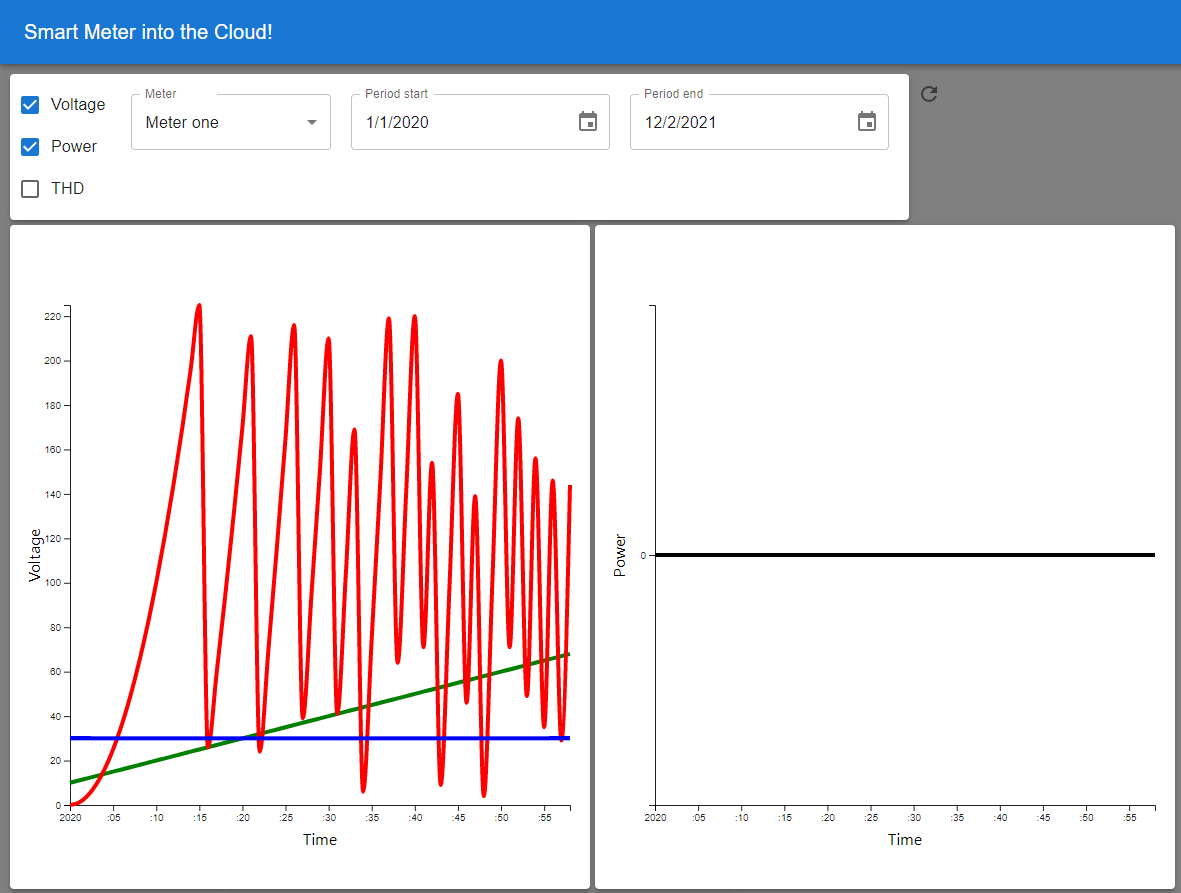
\includegraphics[width=1.0\textwidth]{gfx/phase2}
    \caption{
        Die Benutzerschnittstelle, ausgelegt für Desktop Geräte.
    }
    \label{fig:phase2-ui}
\end{figure}

\subsection{Benutzerschnittstelle}
Um die neuen Anforderungen zur Benutzerschnittstelle zu erfüllen, musste diese neu Entworfen werden.
Das Layout, welches bisher für Mobilgeräte ausgelegt war, konnte sehr einfach für Desktop-Geräte angepasst werden.
In Abbildung \ref{fig:phase2-ui} ist dies zu sehen.
Für die Auswahl eines Zeitintervalls wurden neuen Komponenten oberhalb des Graphen platziert.
Die neuen Leitungs- und \ac{THD} Werte werden in separaten Graphen angezeigt und sind horizontal neben dem bestehenden Graphen angezeigt.
Drei Checkboxen wurden neu hinzugefügt, um die Anzeige der einzelnen Graphen zu steuern.
Ein Dropdown-Menu ermöglicht die Auswahl des Stromzählers, wessen Daten angezeigt werden.
Diese Funktionalität wurde nicht explizit vom Auftraggeber gefordert, war jedoch für das manuelle Testen
und das Demonstrieren der Anwendung sehr praktisch, da so unterschiedliche Daten angezeigt werden können.

\subsection{\ac{API}}
Im vorherigen Abschnitt wurden neue Filter- und Selektionsfunktionen der Benutzerschnittstelle beschrieben.
Damit diese richtig funktionieren, musste auch die \ac{API} entsprechend erweitert werden.
Ein neuer Endpunkt gibt eine Liste aller in der Datenbank vorhandener Stromzähler zurück, so, dass diese für die Auswahl angezeigt werden.
Bei der Anfrage, welche die Messdaten eines bestimmten Stromzählers zurückgibt, kann nun auch ein Zeitintervall mitgegeben werden.

TODO API images

\subsection{Schwierigkeiten}
Schwierigkeiten während der zweiten Iteration
